\documentclass[12pt,a4paper,fleqn]{article}
\usepackage{xcolor}
\usepackage[utf8]{inputenc}
\usepackage{amsmath}
\usepackage{amsfonts}
\usepackage{amssymb}
\usepackage{graphicx}
\usepackage{hyperref}
\usepackage[italian]{babel}
\date{22 luglio 2020}
\author{\\\\\large Marco Balletti, Francesco Marino}
\title{Machine Learning A.A. 2019/2020:\\Relazione Progetto NILM}
\begin{document}
\maketitle

\section{Introduzione}
La presente relazione tratta dei modelli basati su reti neurali proposti per la risoluzione del \textsl{Non-Intrusive Load Monitoring (NILM)}. Lo scopo è quello di realizzare un'architettura di reti neurali in grado di predire, a partire da un valore (espresso in Watt) di consumo energetico totale di un'abitazione, il consumo relativo delle diverse apparecchiature, in particolare, in questo caso, di un frigorifero e di una lavastoviglie. Per la realizzazione del progetto è stato utilizzato \textsl{Python}, come linguaggio di programmazione, affiancato alle librerie \textsl{Numpy} (per la gestione efficiente di \textsl{array} di dati), \textsl{Pandas} (per il reperimento dei dati), \textsl{Tensorflow} e \textsl{Keras} (per la realizzazione e l'addestramento dell'architettura). La piattaforma di sviluppo utilizzata è \textsl{Google Colab} che mette a disposizione degli utenti la possibilità di addestrare delle reti neurali utilizzando anche delle \textsl{GPU} remote.

\section{I dati}
Per la realizzazione del progetto sono stati forniti tre  \textsl{dataset}: il primo contiene i consumi dell'intera abitazione presa in esame registrati con una granularità pari ad un secondo, il secondo ed il terzo contenenti, invece, i consumi relativi al frigorifero e alla lavastoviglie registrati con la stessa granularità e nello stesso intervallo temporale del primo \textsl{dataset}. 
Visto l'ampio quantitativo di dati e la loro dimensione, si è ritenuto conveniente eseguirne il caricamento su \textsl{GitHub} in formato compresso (\texttt{.zip}), tale scelta è motivata anche dalla semplicità con cui, utilizzando \textsl{Python}, \textsl{Keras} e \textsl{Pandas}, è possibile trasformare un \textsl{dataset} compresso in un \textsl{dataframe}.

\subsection{\textsl{Training}, \textsl{Validation} e \textsl{Test set}}
Per garantire la correttezza dell'addestramento del modello e poterne valutare le prestazioni, è stato realizzato lo \textsl{split} del \textsl{dataframe} ricavato precedentemente in \textsl{training set}, \textsl{validation set} e \textsl{test set}. Il primo è stato utilizzato per eseguire l'addestramento dei modelli, il secondo per monitorarne l'\textsl{overfitting} e l'ultimo per valutare le metriche richieste (l'\textit{energy precision}, l'\textsl{energy recall} e l'\textsl{energy F1}) sul modello e poter confrontare le differenti possibili soluzioni tra loro. Durante la creazione di questi \textsl{set} e la conversione da \textsl{dataframe} ad \textsl{array Numpy}, si pone particolare attenzione al consumo della memoria RAM, vengono, infatti, eliminati tutti i riferimenti alle strutture dati non più necessarie dopo la conversione in modo da permettere al \textsl{garbage collector} di eliminarle e recuperare memoria.

Poiché i dati in questione sono di tipo serie temporali, si è deciso di realizzare il \textsl{validation set} ed il \textsl{test set} con misurazioni che fossero temporalmente successive a quelle presenti all'interno del \textsl{training set}, tale relazione di ordine si mantiene anche tra \textsl{validation} e \textsl{test set}.

\subsection{Normalizzazione}
I dati così suddivisi vengono, quindi, sottoposti a normalizzazione sottraendo loro il valore medio e dividendoli per la deviazione standard, tale procedimento si è rivelato essere una strategia particolarmente efficace per la riduzione dei tempi di addestramento dei modelli. I valori necessari per effettuare questa trasformazione sui dati sono stati calcolati utilizzando il solo \textsl{training set}: si è proceduto, in particolare, calcolando la media e la deviazione standard dei consumi dell'abitazione, del frigorifero e della lavastoviglie su questo \textsl{set} di dati, il \textsl{training set} ed il \textsl{validation set} normalizzati sono stati ottenuti, quindi, andando a sottrarre la media relativa al tipo di dato (totale, frigorifero o lavastoviglie) e dividendo per la corrispondente deviazione standard precedentemente calcolate. Per quanto concerne il \textsl{test set}, l'operazione di normalizzazione è stata svolta solo sui consumi totali (sempre utilizzando i valori ricavati dal \textsl{training set}), non è stato necessario eseguirla sui corrispondenti valori di frigorifero e lavastoviglie poiché i dati ottenuti dalla predizione sul \textsl{set} in questione vengono denormalizzati (moltiplicando per la deviazione standard e sommando la media del \textsl{training set}) prima di eseguire la valutazione delle prestazioni.

\subsection{I generatori}
L'addestramento e la valutazione delle prestazioni di modelli basati su dati di tipo serie temporali richiede l'utilizzo di finestre, queste strutture di dati risultano essere necessarie sopratutto se ci si trova nei casi di predittori \textsl{sequence-to-sequence} o \textsl{sequence-to-point}. Realizzare una finestra temporale nel modo classico (\texttt{for} \textit{loop}) si rivela essere particolarmente sconveniente sia in termini di prestazioni che in termini di consumo di memoria RAM, quest'ultimo aspetto, in particolare, risulta essere maggiormente chiaro se si considerano finestre temporali parzialmente sovrapposte per cui una stessa misurazione, ricadendo in più finestre temporali, viene memorizzata molteplici volte.

Per ovviare a questa problematica ed evitare anche di incorrere in \textsl{crash} dell'\textsl{environment Google Colab}, si è proceduto realizzando dei generatori di dati, particolari strutture in grado di creare dinamicamente (all'accesso dell'elemento) \textsl{batch} di dati. L'idea alla base della realizzazione di queste strutture è quella di eseguire un addestramento basato su \textsl{batch} di finestre temporali, quando ne viene richiesto uno nuovo, il generatore determina gli indici degli elementi che faranno parte di ogni singola finestra appartenente al \textsl{batch} (le dimensioni di questo e della finestra sono parametri della struttura, lo scorrimento delle finestre è pari a un elemento), genera le finestre richieste e restituisce l'insieme di dati. Il risparmio di memoria è dovuto al fatto che questo approccio permette di istanziare le sole finestre necessarie in ogni momento, quelle appartenenti a \textsl{batch} precedenti, invece, perdendo ogni riferimento, possono essere deallocate dal \textsl{garbage collector} mantenendo l'utilizzo della RAM costante.

\section{Il modello finale proposto}

Per la predizione dei valori di consumo del frigorifero e della lavastoviglie è stata utilizzata una modifica del \href{https://arxiv.org/abs/1612.09106}{modello \textsl{sequence-to-point} proposto da Zhang}.
Il modello applica alla finestra in input cinque layer Convoluzionali (ognuno, a parte l'ultimo, seguito da un layer di \textsl{Max Pooling}), esegue il \textsl{Dropout} ed il \textsl{Flatten} dei risultati per poi sottoporli a due \textsl{layer Dense} intervellati da un \textsl{Dropout}.

Nel caso del frigorifero è stata utilizzata una finestra temporale di input contenente 2400 misurazioni (40 minuti), nel caso della lavastoviglie, invece, la finestra ha ampiezza di TODO:TOT elementi.


\begin{figure}
\centering
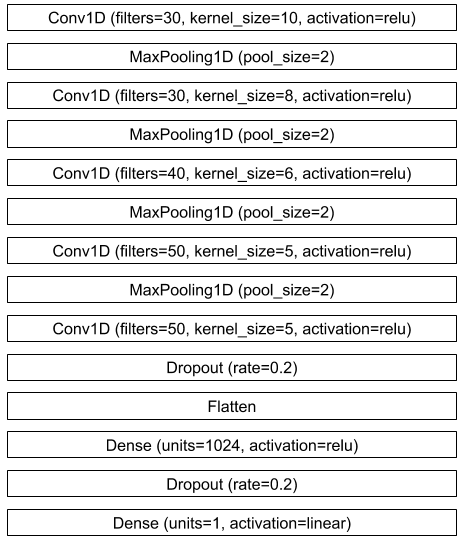
\includegraphics[width=0.5\textwidth]{images/model.png}
\caption{Rappresentazione grafica delle rete neurale utilizzata per le due apparecchiature}
\label{fig:modello}
\end{figure}

\subsection{\textsl{Cross Validation}}
Per determinare le lunghezze delle finestre da utilizzare per ognuna delle apparecchiature, è stata scelta la tecnica della \textsl{cross validation}; per confrontare i risultati, gli addestramenti sono stati effettuati con \textsl{early stopping} (\textsl{patience} = 5) su 15 epoche (quantitativo inferiore rispetto a quello scelto per l'addestramento finale). Per il frigorifero sono state testate finestre di 2000, 2200, 2400 e 2600 elementi (i valori scelti dipendono anche dalla struttura del \textsl{data set}), mentre, per la lavastoviglie, finestre di dimensione 600, 700, 800, 900 e 1000 elementi.

\subsection{Addestramento}
Una volta scelte le lunghezze delle finestre, il modello è stato addestrato in 100 epoche e con \textsl{early stopping} (\textsl{patience}=5), l'ottimizzatore scelto è \textsl{Adam} con funzione di \textsl{loss} la \textsl{mean squared error}. Come anticipato nei paragrafi precedenti, i dati utilizzati per l'addestramento e la valutazione del modello sono stati prodotti utilizzando dei generatori a partire dal \textsl{data set} iniziale, questi, trovandoci nel caso di \textsl{sequence-to-point} con predizione la mediana della finestra, sono stati configurati per porre all'inizio e alla fine del \textsl{set} di dati dei \textsl{dummy values} (elementi pari a 0) in modo tale da creare tante finestre quanti sono gli effettivi valori da predire e facendo sì che al punto mediano di ognuna corrispondesse il corretto valore da ottenere.

Per garantire una maggiore velocità di convergenza dell'algoritmo, è stato utilizzato eseguito un \textsl{reshuffling} dei dati all'inizio di ogni epoca di addestramento.

Sono state salvate due versioni del modello, una addestrata sui dati del frigorifero ed una addestrata sui dati della lavastoviglie, e valutate utilizzando la metrica di \textsl{energy F1}, i risultati ottenuti sono:

\begin{tabbing}
\hspace{2.50in}     \= \hspace{1.00in}		\kill
\textsl{energy F1} per il frigorifero: \> \texttt{0.000000000000}\\
\textsl{energy F1} per la lavastoviglie: \> \texttt{0.000000000000}
\end{tabbing}

\subsection{Alternative testate}

\subsubsection{Modelli alternativi}
Prima di giungere alla soluzione finale proposta, sono stati eseguiti confronti tra differenti architetture (evitando di effettuare \textsl{tuning} dei parametri per ognuna), in particolare, è stato testato l'utilizzo di \href{https://arxiv.org/abs/1507.06594}{\textsl{Denoising Autoencoder (dAE)}}, del \href{https://arxiv.org/abs/1612.09106}{modello \textsl{sequence-to-point} "puro" proposto da Zhang} e del \href{http://nilmworkshop.org/2018/proceedings/Poster_ID20.pdf}{modello proposto dall'organizzazione CSEM} (in particolare, la soluzione finale per il frigorifero prende spunto dagli ultimi due \textsl{paper} riportati).

\subsubsection{\textsl{Downsampling}}
Il confronto del \textsl{data set} fornito per l'esecuzione del progetto con i \textsl{set} di dati utilizzati in letteratura ha evidenziato una forte differenza sulla granularità dei dati: il primo si compone di misurazioni prese ogni secondo, i secondi, tipicamente, di misure intervallate di sei secondi. Alla luce di questa differenza, si è provato a realizzare un \textsl{downsampling} all'interno delle finestre di dati restituite dai generatori in modo tale che, mantenendo fissa la dimensione, l'intervallo temporale coperto dalla finestra fosse maggiore. Questo approccio consente di evitare di dover rinunciare a priori ad una grande quantità di dati, è stato solamente necessario modificare la logica di costruzione dei batch di finestre affinché ognuna prendesse un elemento ogni sei, si noti che finestre consecutive, in questo modo, però, non avranno dati sovrapposti.

\begin{figure}
\centering
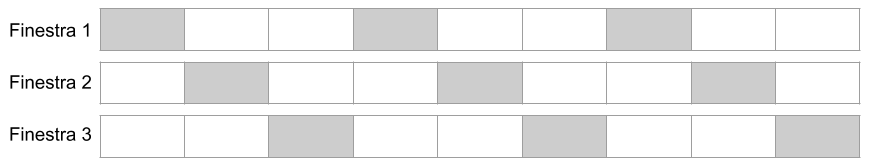
\includegraphics[width=0.8\textwidth]{images/windows.png}
\caption{Rappresentazione grafica della generazione di finestre di dati con \textsl{downsampling}}
\label{fig:finestre}
\end{figure}

Questo tipo di approccio si è rivelato non essere l'ideale per le reti scelte come soluzione finale e, quindi, si è rinunciato ad applicarlo.

\end{document}